\documentclass[11pt]{article}
\usepackage[margin=1in]{geometry}
\usepackage{amsmath,amssymb}
\usepackage{graphicx}
\usepackage{booktabs}
\usepackage{multirow}
\setlength{\emergencystretch}{3em}
\usepackage{listings}
\usepackage{xcolor}
\usepackage[hidelinks]{hyperref}
\lstset{basicstyle=\ttfamily\scriptsize,breaklines=true,columns=fullflexible,keepspaces=true,frame=single,literate={\\}{{\char92}}1 {\$}{{\char36}}1 {\{}{{\char123}}1 {\}}{{\char125}}1 {−}{{-}}1 {×}{{x}}1 {±}{{+-}}1 {·}{{.}}1 {≤}{{<=}}1 {≥}{{>=}}1 {–}{{--}}1}
\newcommand{\grade}[1]{\textsf{\small[#1]}}
\title{When the Neutrinos Leave:\\ Decoupling History and the Threshold for Primordial Black Hole Formation}
\author{Jeromie Beasley}
\date{4 November 2026 \quad (version 4.1)}
\begin{document}
\maketitle

\noindent\emph{AI-assisted. The ideas and research direction are the author's; AI tools (Claude, Anthropic) were used for literature search, computation, drafting and typesetting. The numbers come from the scripts, run logs and outputs printed in Appendix~B. The simulations are runs of S.~McCormick's public code on a cloud computer, not experiments.}

\begin{abstract}
McCormick has shown that neutrinos which stream freely out of a collapsing overdensity raise the threshold for primordial black hole formation, by about $0.235\,R_\nu$ in the linear compaction, and that the effect fades when the neutrinos decouple gradually. This paper asks what sets that fading. First, the neutrino collision operator is read exactly as a cut between what is kept and what streams. All of its non-normality, $\tfrac18\lVert[L,L^\ast]\rVert^2=\kappa^2k^2/3$, lies on the single link between density and flux. With separate rates for flux and shear it is $k^2\kappa_1^2/3+\tfrac{4k^2}{15}(\kappa_2-\kappa_1)^2$, and the weight across the cut equals the sound speed, $\sqrt{E_B}=k/\sqrt3$. Second, McCormick's own code is run on five cases outside his paper, with every prediction and kill line written down before the runs. A broad profile that collapses near $\epsilon\approx7$--$9$ keeps the same share of the neutrino effect as a Gaussian that collapses near $\epsilon\approx4$, or less ($G=0.181$ and $0.045$ against $0.190$ and $0.063$), so the collapse time alone does not set the clock. A steeper decoupling history, $\kappa/H=(\epsilon_{\rm dec}/\epsilon)^6$, gives $G=0.648$, $0.317$ and $0.154$ at $\epsilon_{\rm dec}=1$, $2$ and $3$, against $0.683$, $0.431$ and about $0.30$ for the standard history: how the neutrinos leave matters, not only when. The steep-history thresholds are unchanged by a tenfold higher collision-rate cap and by a finer grid. One reading survives every run: the memory of the kept sector, the population the density keeps under the decoupling operator, read mostly at the first compaction maximum. With one weight fitted to McCormick's curve and then frozen, it predicted $0.663$, $0.246$ and $0.118$ before the runs, all within the kill line of $0.08$; a history-blind rule fails at $\epsilon_{\rm dec}=3$ by $0.146$. Third, the memory has a location. Two neutrino states with the same density, flux and anisotropic stress, differing only in finer angular structure, give later density, flux and stress that differ by several per cent, when the difference is set at or after decoupling; set deep in the coupled era it is erased, by the factor $\exp[-\epsilon_{\rm dec}^n/(n\tau_s^n)]$. An exact block elimination puts the whole effect in one hidden-source term, and the kept population obeys $(\dot A)^2\le4E_BA(1-A)$. A closure on density, flux and stress cannot carry this memory. Fourth, the anisotropic stress sets the threshold. With the flux relaxing at $\kappa_1$ and the shear and every higher moment at $\kappa_2=r\kappa_1$, nine thresholds from $r=1/16$ to $16$ show that the surviving share is not set by the connection energy, which is stationary at $r=1$, but by the direction of the flux--shear mismatch, its reflection coefficient $\Gamma_{12}=(\kappa_2-\kappa_1)/(\kappa_2+\kappa_1)$: $G$ runs from $0.776$ to $0.129$, and its offset $\ln[(1-G)/G]$ moves close to a straight line in the link rapidity $\tfrac12\ln r$, at a rate of $1.113\pm0.007$ near the matched link. Damping the shear alone, with every higher moment left at the flux rate, gives a larger rate, $1.204$, where any rule built from link-weight ratios predicts less than $0.1$: the threshold reads the shear itself. The frozen memory form misses this effect entirely. Halving the neutrino fraction to $R_\nu=0.2$ leaves $G$ at $0.409$, against $0.425$ at $R_\nu=0.409$ measured with the same code. The algebraic identities, the counterexample and the verdict arithmetic are machine-checked in Lean (Appendix~C). Two further tests are stated for the e$^\pm$ annihilation epoch and for the mean of the rates.
\end{abstract}

\section{The question}

Primordial black holes heavier than about $10^6\,M_\odot$ form while the neutrinos, which carry 41--49\% of the radiation, stop scattering and stream freely. McCormick evolved these neutrinos with their angle-resolved transport equation inside spherical general relativity and found that free streaming makes collapse harder~\cite{McC}. The threshold on the linear compaction $C_l$, which sets abundance, rises by $\Delta C_{l,c}/C_{l,c}\simeq0.235\,R_\nu$, and the threshold $\delta_c$ on the compaction peak rises by $\simeq0.15\,R_\nu$. For Gaussian fluctuations a perfect-fluid collapse probability $\beta$ becomes about $\beta^{1.18}$ above $6\times10^5\,M_\odot$.

He also ran gradual decoupling, with collision rate $\kappa=H(\epsilon_{\rm dec}/\epsilon)^3$, where $\epsilon=1/(aHr_m)$ is the Hubble radius in units of the perturbation size. Write $G$ for the share of the instantaneous free-streaming shift that survives:
\begin{equation}
G=\frac{\delta_c-\delta_c^{\rm fluid}}{\delta_c^{\rm inst}-\delta_c^{\rm fluid}}.
\end{equation}
His Table~II gives $G=$ 0.959, 0.867, 0.683, 0.431, 0.190 and 0.063 at $\epsilon_{\rm dec}=$ 0.25, 0.5, 1, 2, 4 and 8. He notes that linear theory gives estimates of opposite sign and ``does not determine which diagnostic, if any, predicts the nonlinear threshold''~\cite[Sec.~IV\,C]{McC}.

Two questions follow and are answered here. What in the neutrino transport operator carries the effect (Section~\ref{sec:cut})? And which clock, and which part of the decoupling history, sets $G$ (Sections~\ref{sec:runs}--\ref{sec:memory})?

\section{The collision operator as a cut}\label{sec:cut}

For one Fourier mode $k$, the linearised neutrino intensity in McCormick's relaxation model evolves under
\begin{equation}
\partial_t f=L f,\qquad L=A+D,\qquad A=-ik\mu,\qquad D=-\kappa(I-P),
\end{equation}
where $\mu$ is the cosine of the angle to the wave vector and $P$ projects onto the isotropic part. Free streaming $A$ is anti-Hermitian. Collisions $D$ are Hermitian, conserve the isotropic part (the neutrino energy in the plasma frame) and remove the flux, which goes to the plasma. In the normalised Legendre basis $|\ell\rangle$, streaming couples only neighbours, $\langle\ell+1|\mu|\ell\rangle=c_\ell=(\ell+1)/\sqrt{(2\ell+1)(2\ell+3)}$, so the operator lives on a chain $\ell=0,1,2,\dots$ (Figure~\ref{fig:chain}).

\paragraph{Non-normality is connection energy.} For Hermitian $D$ and anti-Hermitian $A$, $[L,L^\ast]=2[A,D]$, and for diagonal $D$, $[A,D]_{ij}=A_{ij}(D_j-D_i)$. Hence
\begin{equation}
\tfrac18\lVert[L,L^\ast]\rVert_F^2=\sum_{\text{links }\ell\to\ell+1}k^2c_\ell^2\,(D_{\ell+1}-D_\ell)^2 .
\end{equation}
This is the scalar case of the identity in~\cite{CE}: the self-commutator energy of a transport operator is the energy of its Hermitian field failing to be parallel along the links \grade{derived; Appendix A.1}. With one rate, only the link $0\to1$ has a jump, so
\begin{equation}
\tfrac18\lVert[L,L^\ast]\rVert_F^2=\frac{\kappa^2k^2}{3}\qquad\text{\grade{derived; checked to $10^{-12}$, I1}}.
\end{equation}
All the non-normality of the single-rate model lies on the link between density and flux, the same channel as the momentum drag $\kappa q$ in McCormick's plasma equation~\cite[Eq.~(6)]{McC}.

\paragraph{Beyond relaxation time.} Let the flux relax at $\kappa_1$ (momentum transfer) and shear and higher moments at $\kappa_2$. Then two links carry jumps:
\begin{equation}
\tfrac18\lVert[L,L^\ast]\rVert_F^2=\frac{k^2\kappa_1^2}{3}+\frac{4k^2}{15}(\kappa_2-\kappa_1)^2\qquad\text{\grade{derived; checked, I2}}.
\end{equation}
The energy is stationary in $\kappa_2$ at $\kappa_2=\kappa_1$. If neutrino--neutrino scattering damps shear but not flux, with rates relative to e$^\pm$ scattering of $1.5$ for $\nu_e$ and $7$ for $\nu_{\mu,\tau}$, the shear link carries 64\% and 97.5\% of the non-normality \grade{computed, under those assumed ratios}.

\paragraph{The weight across the cut is the sound speed.} With $H=k\mu$ the weight between kept and streaming parts is $E_B=\lVert PH(I-P)\rVert^2=k^2c_0^2=k^2/3$, so $\sqrt{E_B}=k/\sqrt3=c_s k$, the radiation sound speed~\cite{WB} \grade{derived; I3}. A rate bound built on $E_B$ therefore sees the root-mean-square streaming speed $1/\sqrt3$, not the light-speed front that empties the overdensity~\cite{OSL}.

\paragraph{The kept sector, exactly.} The isotropic part has the closed propagator
\begin{equation}
\langle0|(s-L)^{-1}|0\rangle=\frac{g}{1-\kappa g},\qquad g=\frac1k\arctan\frac{k}{s+\kappa}\qquad\text{\grade{derived; checked, I4}}.
\end{equation}
The two-moment truncation, keeping $\ell=0,1$, has eigenvalues $-\kappa/2\pm\sqrt{\kappa^2/4-k^2/3}$, which merge at $\kappa=2k/\sqrt3$ \grade{derived; I5}. This exceptional point belongs to the truncation. With 200 moments the least-damped mode turns real only at $\kappa\approx0.646\,k$, and in relaxation kinetic theory the hydrodynamic poles meet a branch cut instead~\cite{Rom,Hu} \grade{computed}.

\begin{figure}[t]\centering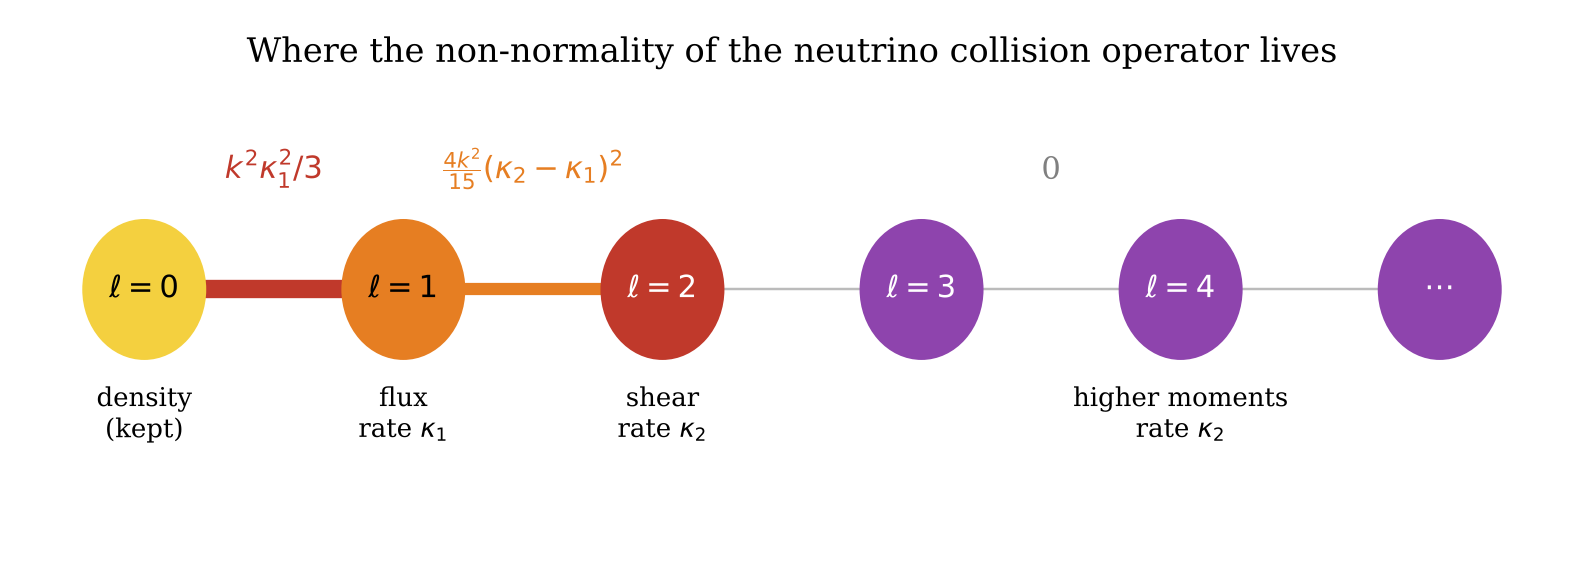
\includegraphics[width=0.95\textwidth]{figs/fig2_chain.png}
\caption{The neutrino moments form a chain. Streaming links each moment to its neighbours; collisions put a rate on each. Non-normality sits only where neighbouring rates differ: on the density--flux link ($k^2\kappa_1^2/3$) and, if shear relaxes at its own rate, on the flux--shear link. Every other link carries none.}\label{fig:chain}\end{figure}

\section{New runs of McCormick's code}\label{sec:runs}

The code~\cite{McCcode} was run unchanged except for one copied file in which the decoupling exponent $n$ in $\kappa=H(\epsilon_{\rm dec}/\epsilon)^n$ is an input. Pure radiation, $R_\nu=0.409$, $N=400$ cells, $N_\mu=32$ angle bins, $\epsilon_0=0.1$, as in his Table~II. A reproduction run at $\delta=0.5109$ with $n=3$, $\epsilon_{\rm dec}=2$ forms a black hole, inside his published bracket $(0.51074,0.51109)$ \grade{measured; Appendix B.4}. For the steep history, $\kappa/H$ was capped at $5\times10^5$, the stiffness his own $\epsilon_{\rm dec}=8$ runs reach at $\epsilon_0$. At that cap deviations from isotropy are of relative order $H/\kappa\le2\times10^{-6}$, the same estimate McCormick uses for his switch to transport~\cite[Sec.~III]{McC}.

For every test below each prediction and its kill condition were written before the runs (Appendix~B.3). The threshold search runs two points per round; a run that neither collapses nor disperses by the end time, or that stops on an error, never moves the bracket, is retried once with a longer end time and is reported if still undecided. No point in any run below was undecided.

\paragraph{Test A: a profile that collapses late.} The broad profile $\alpha=0.3$ is decided near $\epsilon\approx7$--$9$, against $\epsilon\approx4$ for the Gaussian. Its thresholds are $\delta_c^{\rm fluid}=0.44805$ and $\delta_c^{\rm inst}=0.47747$~\cite{McCcode}. With $n=3$:
\begin{center}\begin{tabular}{lccc}\toprule
& $\delta_c$ & $G$ (broad) & $G$ (Gaussian, \cite{McC}) \\\midrule
$\epsilon_{\rm dec}=4$ & $0.45337\pm0.00013$ & $0.181\pm0.004$ & $0.190$\\
$\epsilon_{\rm dec}=8$ & $0.44938\pm0.00012$ & $0.045\pm0.004$ & $0.063$\\\bottomrule\end{tabular}\end{center}
The broad profile keeps the same share of the neutrino effect as the Gaussian or less (29\% less at $\epsilon_{\rm dec}=8$), although it collapses about twice as late (Figure~\ref{fig:clock}) \grade{measured}. A clock tied to the collapse time would have raised $G$; it fell. Because the test changes the profile shape together with the collapse time, it shows that the collapse time alone does not set the clock; it does not by itself separate the two, and it does not fix which earlier epoch does.

\paragraph{Tests B, C and D: a steeper decoupling history.} Gaussian profile, $\kappa/H=(\epsilon_{\rm dec}/\epsilon)^6$:
\begin{center}\begin{tabular}{lccc}\toprule
& $\delta_c$ & $G$ ($n=6$) & $G$ ($n=3$, \cite{McC}) \\\midrule
C: $\epsilon_{\rm dec}=1$ & $0.51756\pm0.00019$ & $0.648\pm0.006$ & $0.683$\\
B: $\epsilon_{\rm dec}=2$ & $0.50743\pm0.00011$ & $0.317\pm0.004$ & $0.431$\\
D: $\epsilon_{\rm dec}=3$ & $0.50245\pm0.00019$ & $0.154\pm0.006$ & $\approx0.30$\\\bottomrule\end{tabular}\end{center}
\grade{measured}. The $n=3$ value at $\epsilon_{\rm dec}=3$ lies between McCormick's $0.431$ and $0.190$ at 2 and 4. A neutrino population that decouples more abruptly, but by the same nominal time, keeps less of its effect, and the gap widens with $\epsilon_{\rm dec}$. The history matters, not only its end point.

\paragraph{Numerical controls.} Test B was repeated with the rate cap raised tenfold, to $5\times10^6$, and on a finer grid, $N=600$ cells and $N_\mu=48$ angle bins. The thresholds are $\delta_c=0.50740\pm0.00011$ and $0.50751\pm0.00006$, shifts of $-0.00003$ and $+0.00008$ against the pre-registered tolerance of $0.0005$ \grade{measured}. The cap acts only while the neutrinos are tightly coupled: the uncapped rate starts at $(\epsilon_{\rm dec}/\epsilon_0)^6$ and falls below the cap at $\epsilon\approx0.11$, $0.22$ and $0.34$ for $\epsilon_{\rm dec}=1$, 2 and 3. The cap control was run at $\epsilon_{\rm dec}=2$ only; at $\epsilon_{\rm dec}=1$ and 3 it is untested.

\begin{figure}[t]\centering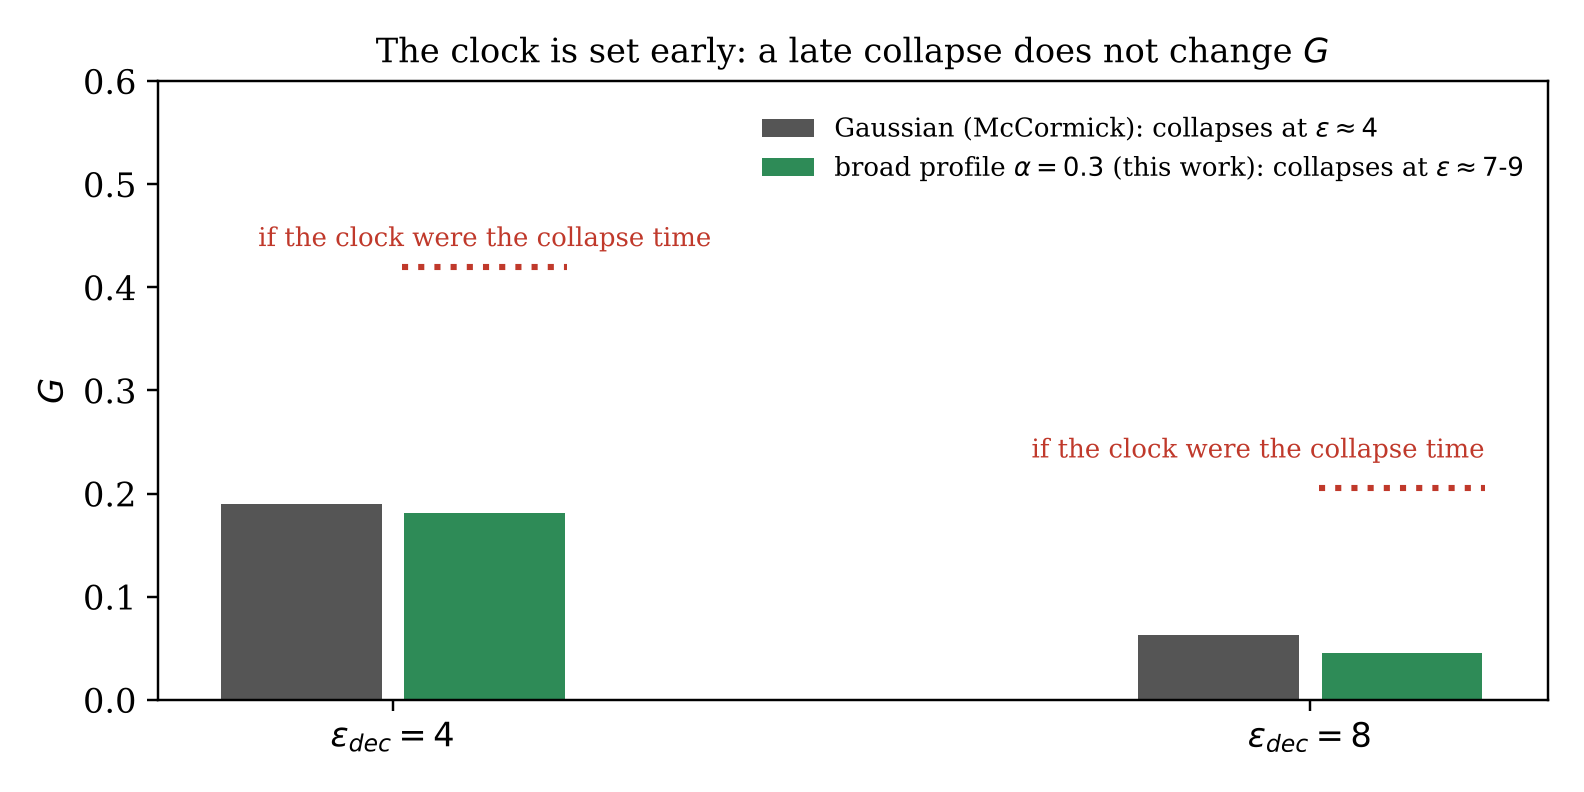
\includegraphics[width=0.9\textwidth]{figs/fig3_clock.png}
\caption{Test A. The broad profile collapses at $\epsilon\approx7$--$9$, yet keeps the same share $G$ of the free-streaming shift as the Gaussian. A clock tied to the collapse time would have given the dotted values.}\label{fig:clock}\end{figure}

\section{What does not set the threshold}\label{sec:not}

Each reading below was tested against numbers. Only the last two were tested against runs set up for them in advance; the first three were tested against McCormick's published curve.

\begin{enumerate}
\item \textbf{The first maximum of linear theory.} The linear density contrast at its first maximum ($\epsilon\approx1.7$) reproduces the instantaneous shift (centre factor $0.944$, as McCormick finds). Under gradual decoupling the share it keeps is 0.86, 0.59, 0.19, $-0.05$, $-0.02$ and 0.00, a largest error of $0.50$. Decoupling after $\epsilon\approx1.7$ is nearly invisible to it, yet still moves the nonlinear threshold \grade{computed}.
\item \textbf{A sharp wall, and rate ratios.} Treat the two-moment exceptional point, crossed at $\epsilon_{\rm EP}=0.811\,\epsilon_{\rm dec}^{3/4}$ for $kr_m=2$, as a wall, or use the parameter-free escape fractions $k/(k+\kappa)$, $e^{-\kappa/k}$ and $1-e^{-k/\kappa}$. Averaging each over two windows, with two weightings and two scales, gives 32 combinations. The wall variants miss by $0.14$ or more. With the window starting at horizon entry, every combination misses by $0.17$ or more. One combination, $e^{-\kappa/k}$ averaged from $\epsilon_0$, comes within $0.077$; selected from 32, it is not counted. On Test B, which it never saw, it predicts $0.513$ against $0.317$ \grade{computed; measured}.
\item \textbf{Diffusive escape.} Diffusion with $D=1/(3\sigma)$ from the conformal rate $\sigma=\epsilon_{\rm dec}^3/\tau^4$, combined in series with streaming at the collapse time $\epsilon^\ast$, gives $G=1/[1+\sqrt{15}(\epsilon_{\rm dec}/\epsilon^\ast)^{3/2}]$. With $\epsilon^\ast=4$ it matches McCormick's curve to $0.02$, but it was built after seeing that curve, and a free fit of its exponent gives $1.61\pm0.03$ rather than $3/2$. Test A with $\epsilon^\ast=7$--$9$ predicted $0.37$--$0.47$ and $0.17$--$0.24$, and Test B predicted $0.62$. Both are excluded \grade{measured}.
\item \textbf{History-blind.} If only $\epsilon_{\rm dec}$ mattered, Tests B and D would give $0.431$ and about $0.30$. They give $0.317$ and $0.154$; Test D misses by $0.146$ against a kill line of $0.08$ \grade{measured}.
\end{enumerate}

\section{What survives: the memory of the kept sector}\label{sec:memory}

The reading that survives treats the isotropic part as a kept sector and asks how much of it the decoupling operator keeps~\cite{WB}. Start a mode in $|0\rangle$ at $\tau_0=0.02$ and evolve it under $\partial_\tau v=-(ik\mu+a\kappa(\tau)(I-P))v$, with $a\kappa=\epsilon_{\rm dec}^n/\tau^{n+1}$. Let $A(\tau)$ be the population left in $|0\rangle$, averaged over the Gaussian profile with weights $k^2e^{-k^2/2}$. Define
\begin{equation}
g(\epsilon^\ast)=\frac{1-A_{\epsilon_{\rm dec}}(\epsilon^\ast)}{1-A_{\rm inst}(\epsilon^\ast)},
\end{equation}
the share of the kept sector's loss that has happened by the readout time $\epsilon^\ast$.

With no fitted number, read at the first compaction maximum $\epsilon^\ast=1.7$, it gives 0.941, 0.860, 0.671, 0.344, 0.087 and 0.013 against McCormick's $G$. That is within $0.02$ for $\epsilon_{\rm dec}\le1$, with a largest error of $0.103$, just outside the $0.10$ bar set for it in advance \grade{computed}. McCormick's own curve passes $G=\tfrac12$ at $\epsilon_{\rm dec}\approx1.67$, within 3\% of the first maximum: the neutrinos must be decoupled by then for half the effect to survive.

The late shortfall says the collapse is still listening after the first maximum. Mixing the two epochs McCormick's numbers single out, $g_2=w\,g(1.7)+(1-w)\,g(4.0)$, with one weight fitted to his curve, $w=0.89$, gives a largest error of $0.022$ \grade{fit}. The form is not unique: with the scale fixed at $kr_m=2$ the single-epoch reading misses by $0.093$, and the best single readout epoch, $\epsilon^\ast=1.87$, by $0.065$. Its weight does not carry over between weightings: the same $w$ with the scale fixed at $kr_m=2$ misses by $0.115$, outside the $0.10$ bar declared for that check \grade{computed}. The form is a fitted shape with a stated sensitivity, not a derived law.

The test is what that fitted form says about histories it never saw. All its $n=6$ values were computed in one file dated 13:47 on 30 October, before any $n=6$ run, and were not refitted afterwards:
\begin{center}\begin{tabular}{lccccc}\toprule
& predicted & measured & miss & history-blind & miss\\\midrule
C: $\epsilon_{\rm dec}=1$ & $0.663$ & $0.648$ & $0.014$ & $0.683$ & $0.035$\\
B: $\epsilon_{\rm dec}=2$ & $0.246$ & $0.317$ & $0.071$ & $0.431$ & $0.114$\\
D: $\epsilon_{\rm dec}=3$ & $0.118$ & $0.154$ & $0.037$ & $\approx0.30$ & $0.146$\\\bottomrule\end{tabular}\end{center}
Every miss of the memory form lies inside the kill line of $0.08$ set before its run; the history-blind rule fails at $\epsilon_{\rm dec}=3$ (Figures~\ref{fig:G} and~\ref{fig:kill}) \grade{measured}. At $\epsilon_{\rm dec}=2$ and 3 the form falls below the measurement: it counts slightly too much of the early erasure. Test C was set where the two rules nearly agree, as a survival check; Test D was set where they separate. A readout window set by the neutrino flux and the enclosed mass between first maximum and apparent horizon, as McCormick suggests~\cite[Sec.~IV\,C]{McC}, is the natural next object. It is untested.

\begin{figure}[t]\centering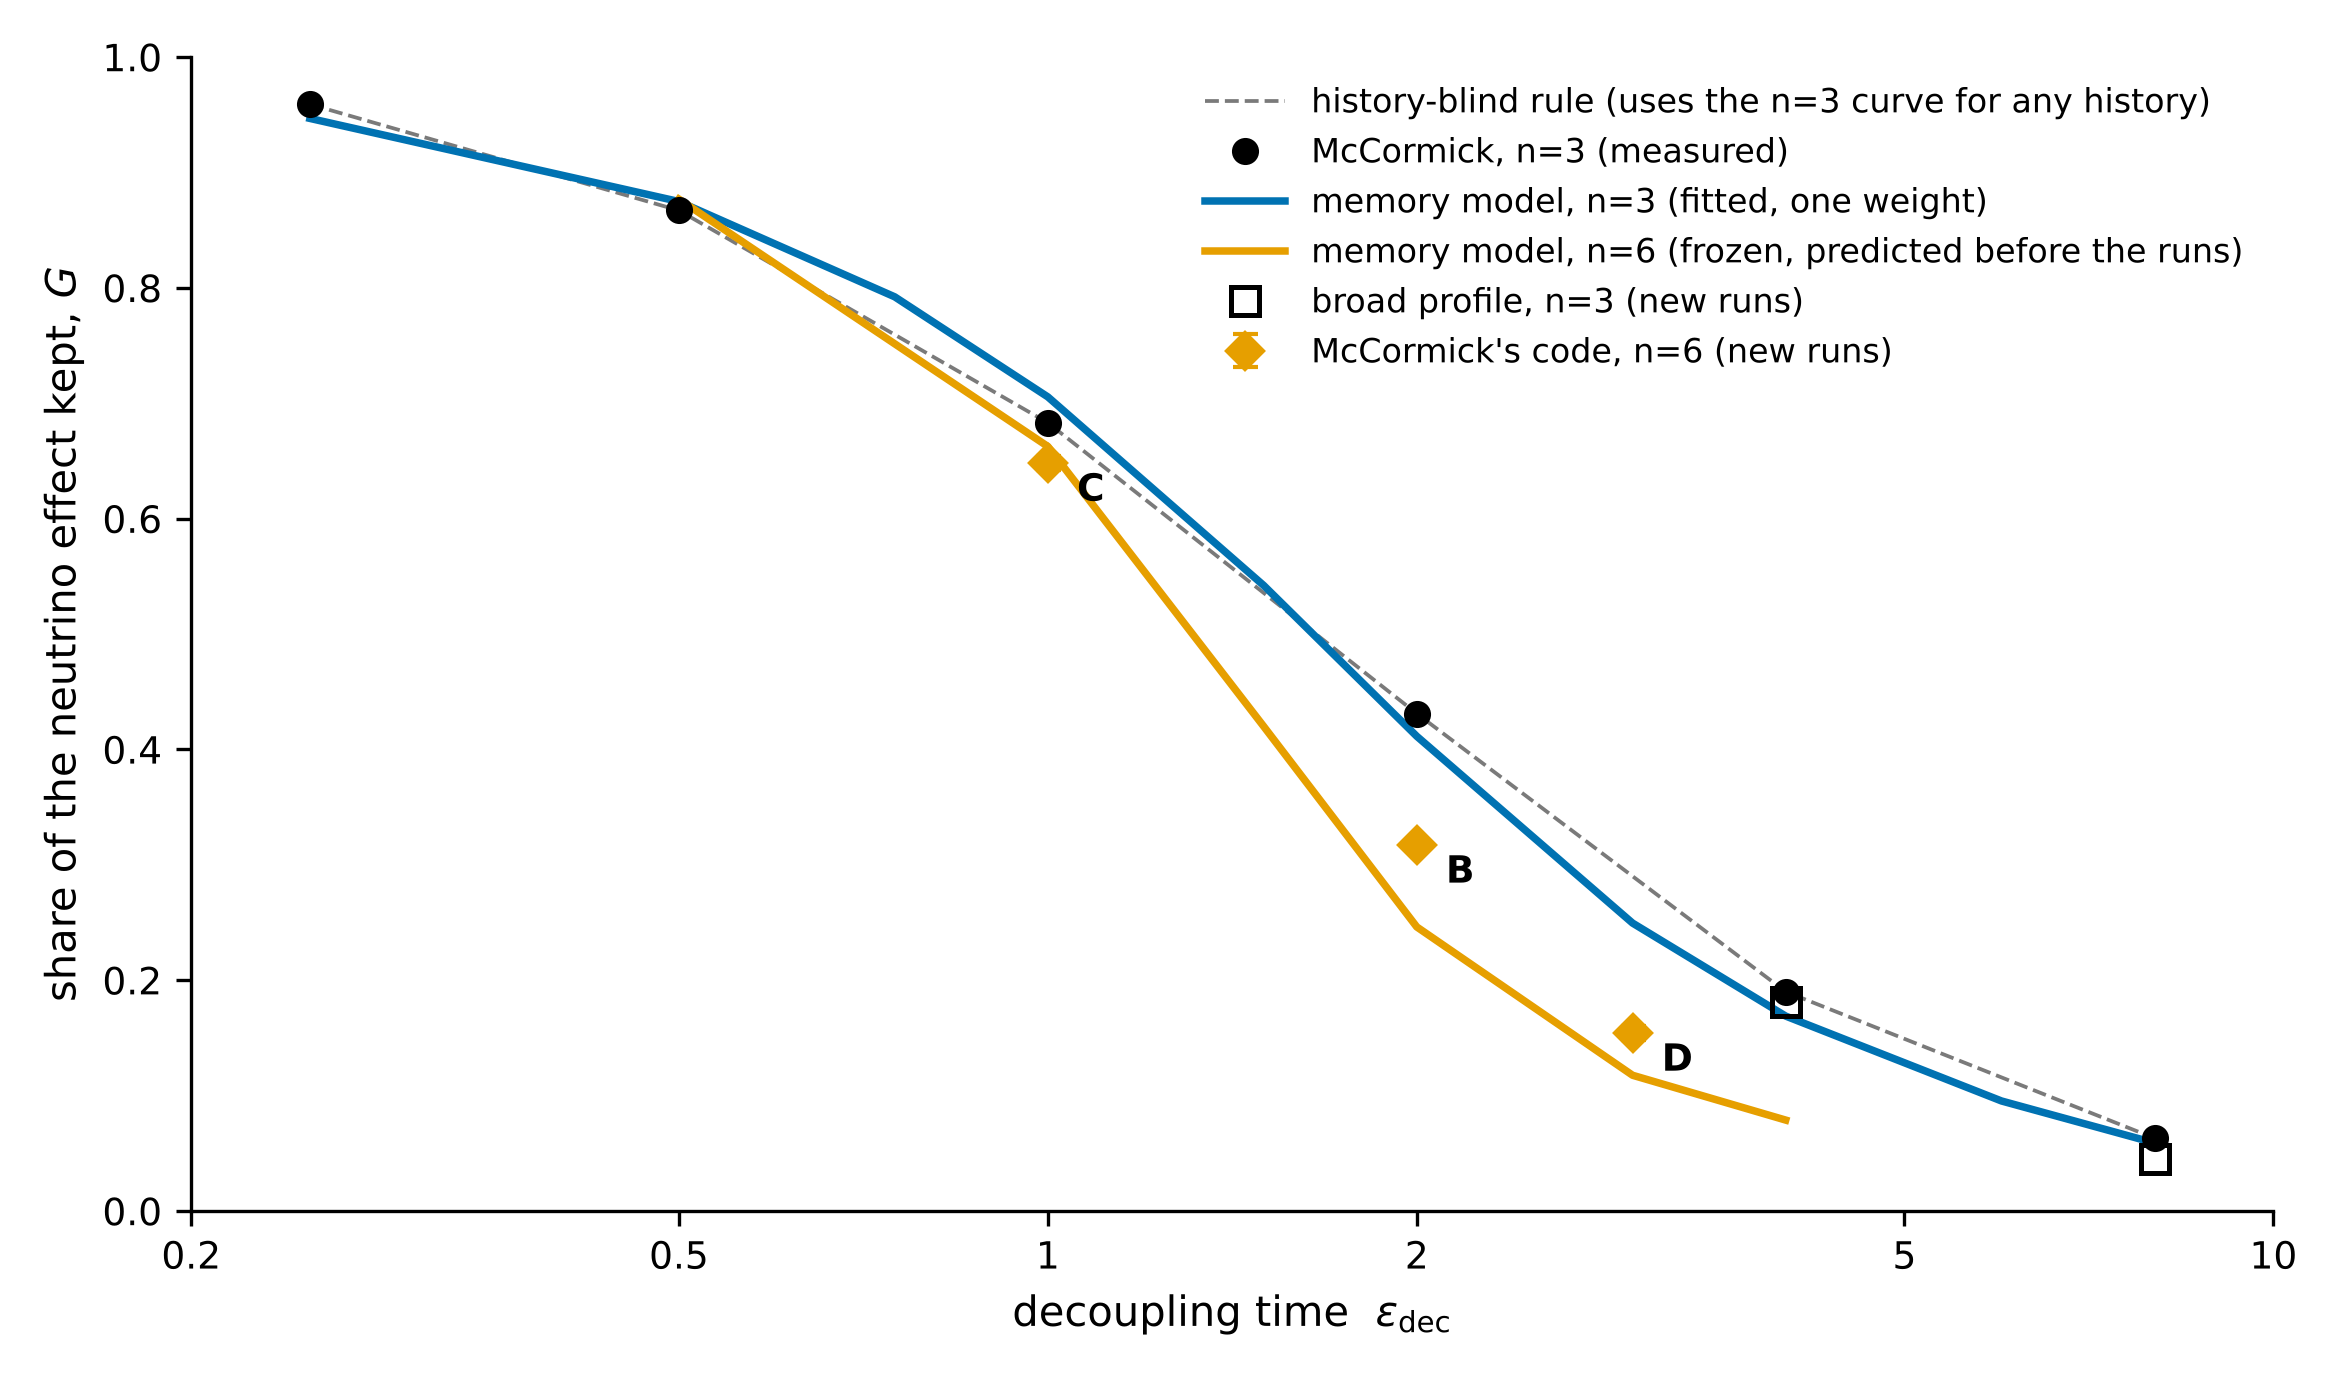
\includegraphics[width=0.95\textwidth]{figs/fig4_tests.png}
\caption{The surviving share $G$ of the free-streaming shift against decoupling time. Black dots: McCormick's Gaussian runs with $\kappa/H=(\epsilon_{\rm dec}/\epsilon)^3$; the grey dashed line through them is what a history-blind rule gives for any history. Blue: the kept-sector memory with one weight fitted to the black dots. Orange line: the same form for $\kappa/H=(\epsilon_{\rm dec}/\epsilon)^6$, computed before any such run and not refitted. Orange diamonds: the new $n=6$ runs C, B and D. Open squares: the broad profile (Test A).}\label{fig:G}\end{figure}

\begin{figure}[t]\centering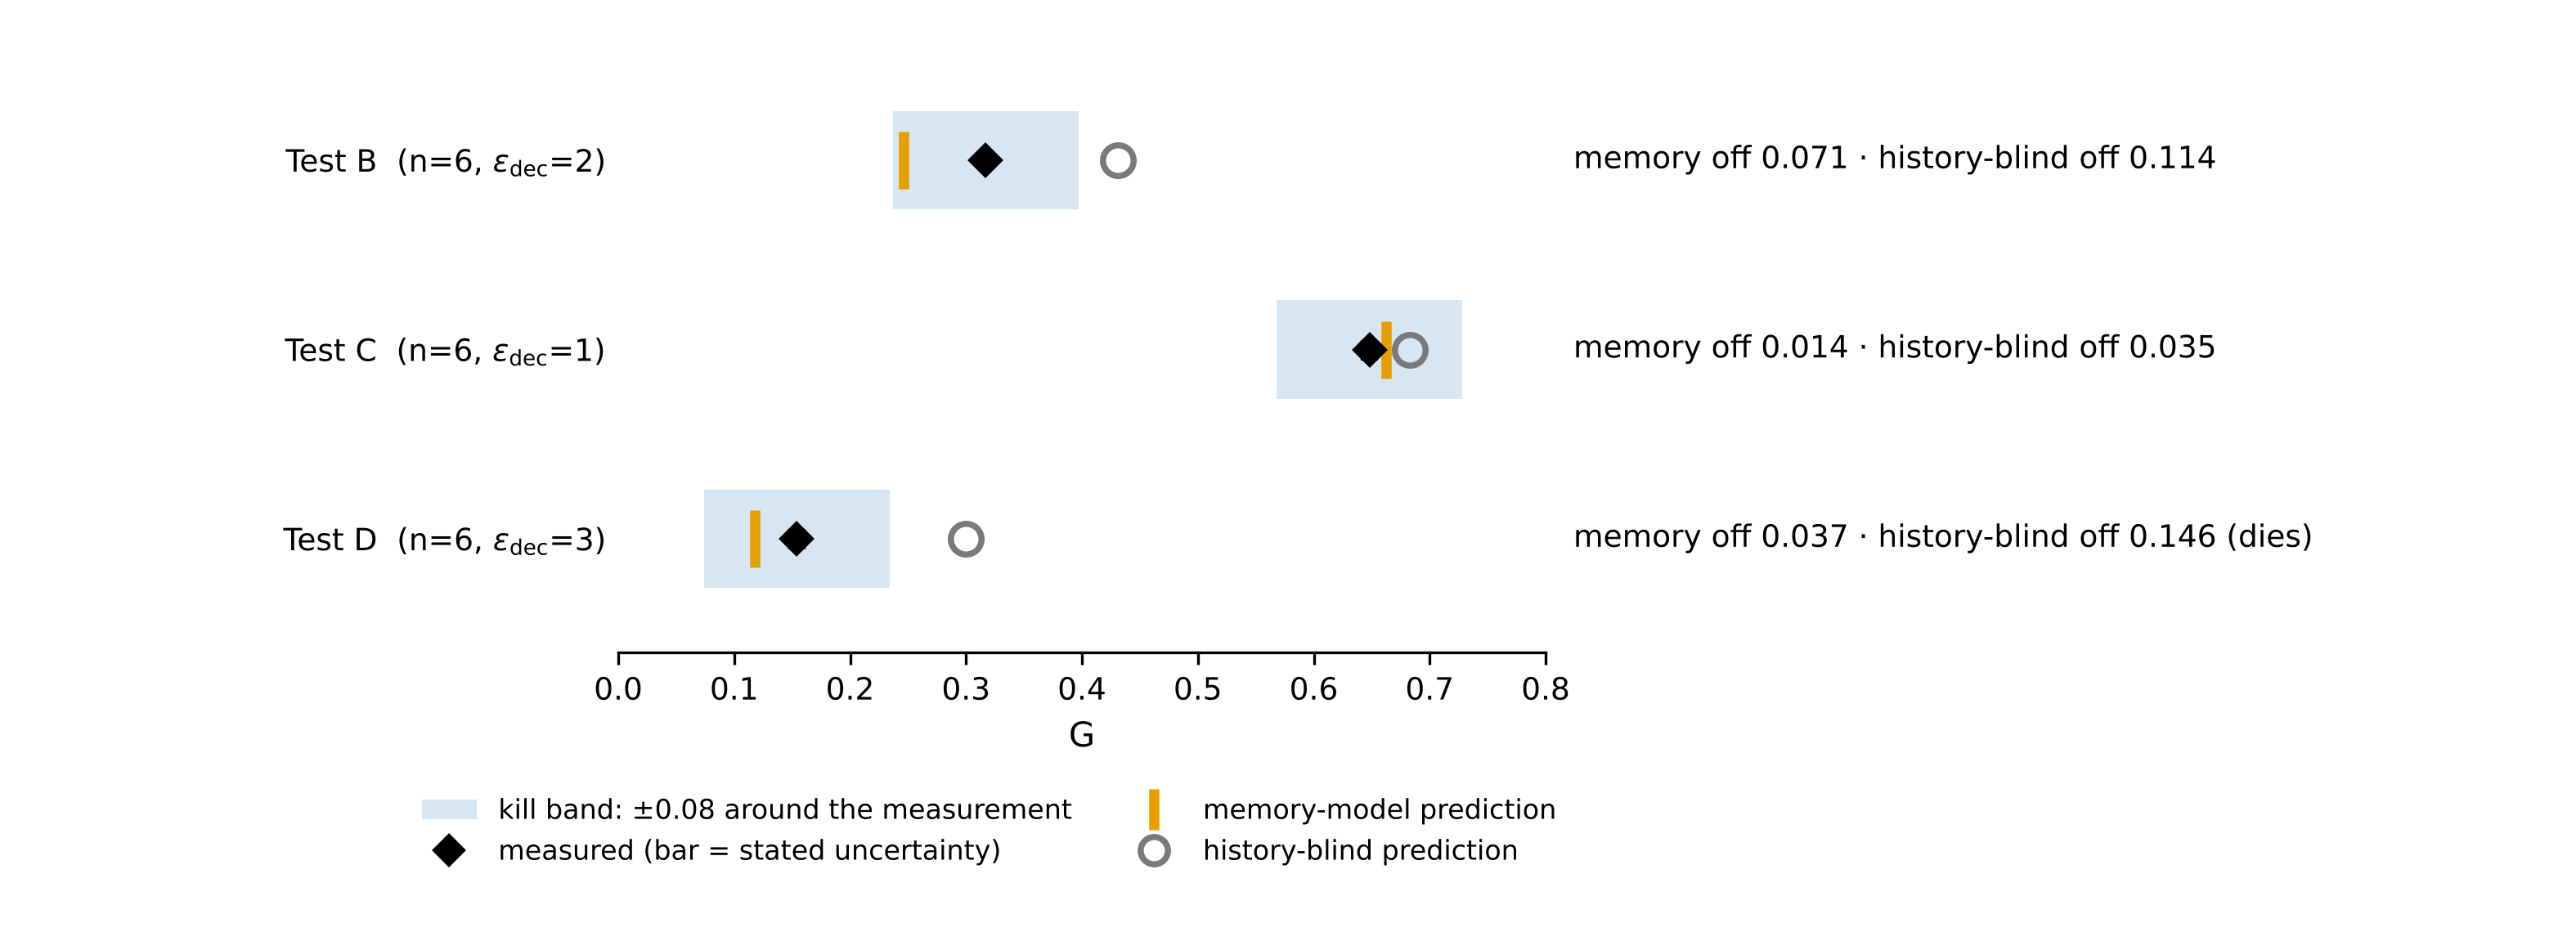
\includegraphics[width=\textwidth]{figs/fig5_killlines.png}
\caption{The three steep-history tests against their kill lines. The shaded band is $\pm0.08$ around each measurement. Orange: the memory form's prediction, made before the run. Grey circle: the history-blind rule. At $\epsilon_{\rm dec}=3$ the history-blind rule falls outside the band.}\label{fig:kill}\end{figure}

\section{Where the memory sits}\label{sec:witness}

A fluid closure carries the density, the flux and the anisotropic stress, the moments $\ell=0,1,2$. The memory form of Section~\ref{sec:memory} says the threshold depends on how the kept sector was emptied. The question here is whether that history can sit in moments a closure does not carry.

\paragraph{Exact elimination of the hidden moments.} Split $v=(a,h)$ with $a=v_0$ and $h=(v_1,v_2,\dots)$. In the relaxation model every hidden moment is damped at the same rate, so the collision term on the hidden block is $\sigma(\tau)$ times the identity and commutes with streaming. The hidden propagator is therefore exact in closed form,
\begin{equation}
U_Q(t,r)=e^{-[\Sigma(t)-\Sigma(r)]}\,e^{-ik(t-r)M_{QQ}},\qquad \Sigma(\tau)=-\frac{\epsilon_{\rm dec}^{\,n}}{n\tau^n},\quad \Sigma'=\sigma,
\end{equation}
and eliminating $h$ gives one equation for the kept amplitude,
\begin{equation}
\dot a(t)=S(t)-k^2\!\int_s^t K(t,r)\,a(r)\,dr,\qquad K=c_0^2\,[U_Q(t,r)]_{11},\qquad S=-ikc_0\,[U_Q(t,s)h(s)]_1
\end{equation}
\grade{derived; Appendix A.5}. The kernel $K$ is the memory; the source $S$ is everything the hidden moments held at time $s$.

\paragraph{The matched pair.} Take two states with the same $(v_0,v_1,v_2)=(1,0.2,0.1)$, differing only by $\pm0.05$ in $v_3$ (or $v_4$), scaled by one constant to unit norm. Both are positive angular distributions ($f(\mu)\ge0.50$). Their kept amplitudes start equal, so their difference obeys the equation above driven only by $S$ of the hidden difference. Both are evolved under the same history, $\epsilon_{\rm dec}=0.5$, with the planting time $\tau_s$ scanned across decoupling. The readout is the profile-weighted change in $(v_0,v_1,v_2)$, relative to its size, $R_{\rm ret}$; the witness is on if $R_{\rm ret}>10^{-3}$. Every on/off call was written down before the run, from the survival factor of the hidden block, $\exp[-\epsilon_{\rm dec}^n/(n\tau_s^n)]$, and the leakage $(k/\sigma)^\ell$ through damped rungs (Appendix~B.14).

\begin{center}\begin{tabular}{lcccc}\toprule
$\tau_s/\epsilon_{\rm dec}$ & $n=3$, $\ell=3$ & $n=3$, $\ell=4$ & $n=6$, $\ell=3$ & $n=6$, $\ell=4$\\\midrule
0.1 & $7\times10^{-15}$ & $5\times10^{-19}$ & $8\times10^{-24}$ & $5\times10^{-31}$\\
0.25 & $6\times10^{-10}$ & $6\times10^{-11}$ & $2\times10^{-15}$ & $7\times10^{-20}$\\
0.5 & $\mathbf{8.6\times10^{-3}}$ & $\mathbf{7.9\times10^{-3}}$ & $3\times10^{-6}$ & $3\times10^{-6}$\\
1 & $\mathbf{0.081}$ & $\mathbf{0.074}$ & $\mathbf{0.094}$ & $\mathbf{0.086}$\\
2 & $\mathbf{0.095}$ & $\mathbf{0.085}$ & $\mathbf{0.098}$ & $\mathbf{0.088}$\\\bottomrule\end{tabular}\end{center}
$R_{\rm ret}$ at $\tau=4$; bold entries are on \grade{computed}. Every call came out as predicted. The survival law is quantitative: for $n=3$ the ratio of the entries at $0.5$ and $1$ is $0.106$ against $e^{-8/3}/e^{-1/3}=0.097$, and for $n=6$ at $0.5$ the law gives $1.4\times10^{-6}$ against $1.6\times10^{-6}$ at $\tau=1.7$. Planted in the retained moments instead, deep in coupling the order is $\ell=1>2>3>4$, each rung costing about $10^{-4}\approx k/\sigma$; after decoupling all four are of the same size. A hidden difference set at decoupling changes the later density, flux and stress as much as a visible one (Figure~\ref{fig:door}).

\paragraph{Checks.} Doubling the number of moments, $60\to120$, and tightening the solver tolerances change every entry by at most $1.4\times10^{-5}$ of its value. Solving the elimination equation from the closed-form $U_Q$ alone, with no solve of the full system, reproduces the full difference to $3\times10^{-7}$--$7\times10^{-7}$, falling fourfold with each halving of the step; leaving out the kernel misses by 19--234\% \grade{computed; Appendix B.14}.

\paragraph{A speed limit on the kept population.} Collisions conserve $|0\rangle$ and remove the rest, so $\lVert v\rVert$ never grows, and streaming links $|0\rangle$ only to $|1\rangle$, with weight $kc_0=\sqrt{E_B}$. Hence for $A=|v_0|^2$
\begin{equation}
\dot A^2\le4E_B\,A(1-A),\qquad E_B=k^2/3
\end{equation}
\grade{derived; Appendix A.6; Lean}. On every trajectory computed here the largest value of the ratio is $0.87$ \grade{computed}. The bound limits how fast the kept sector can be emptied; it does not set the threshold.

\paragraph{Reading.} A closure on density, flux and stress is exact only for structure set while the neutrinos are tightly coupled. Structure set at or after decoupling survives in the finer angular moments and streams back into the visible ones by several per cent. The memory McCormick's runs record therefore has a place to live that no fluid closure contains. Whether realistic initial data carry such structure, and how far it moves the nonlinear threshold, are untested: the memory curves of Section~\ref{sec:memory} start with the hidden moments empty.

\begin{figure}[t]\centering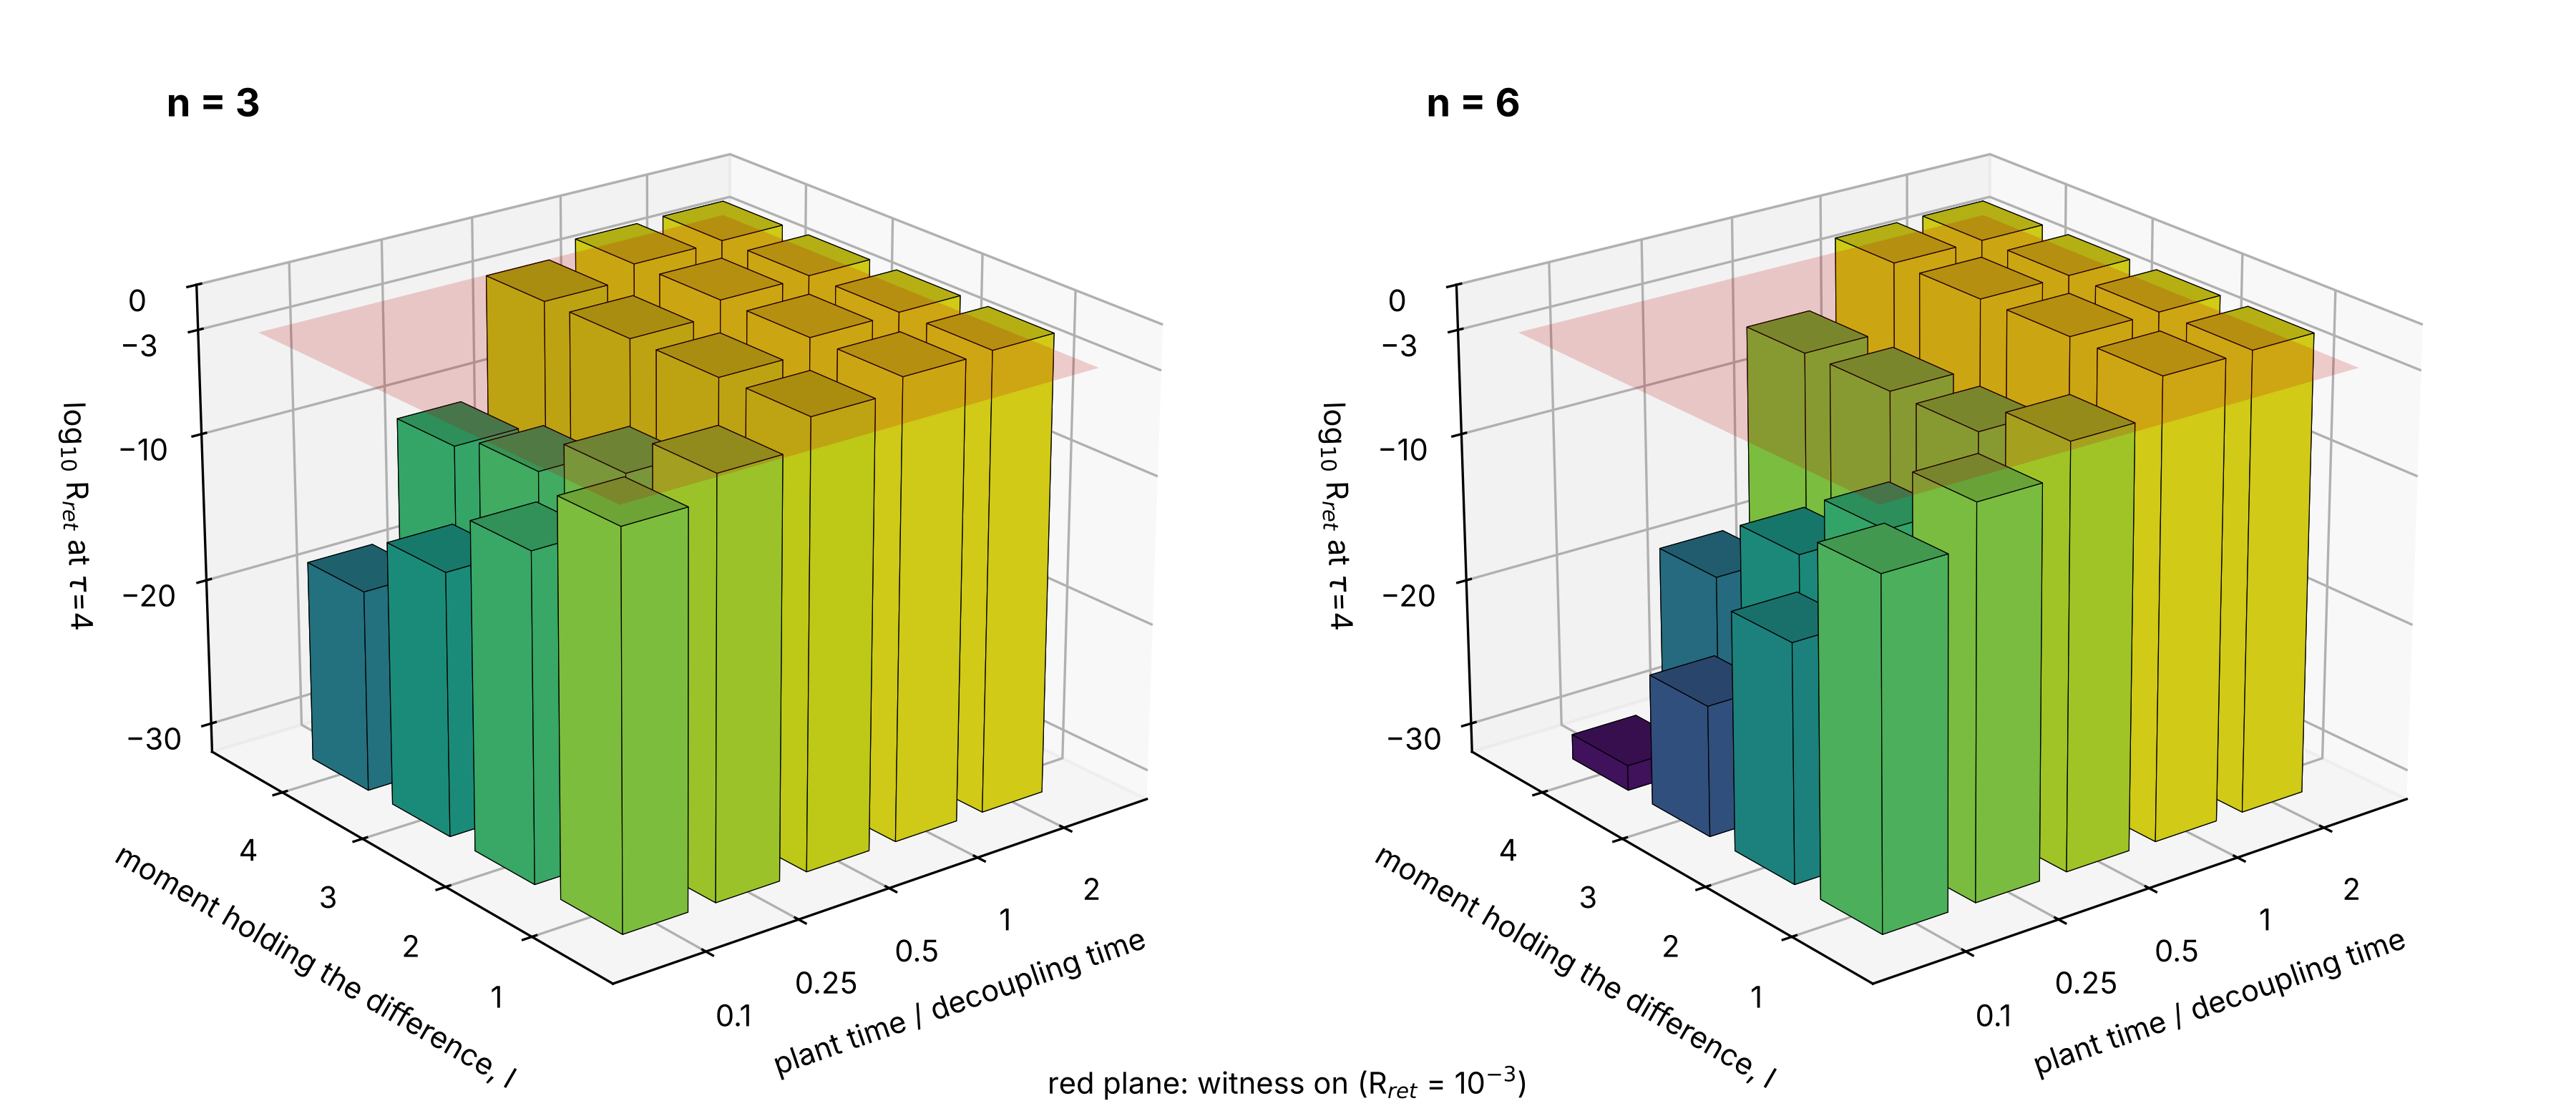
\includegraphics[width=\textwidth]{figs/fig6_door.png}
\caption{The door. Strength of the matched-pair witness, $\log_{10}R_{\rm ret}$ at $\tau=4$, against the time the hidden difference was planted (in units of $\epsilon_{\rm dec}$) and the moment that held it. Planted deep in the coupled era the difference is erased, down to $10^{-30}$; planted at or after decoupling it returns at the $10^{-1}$ level. The red plane is the witness threshold $10^{-3}$. The steeper history ($n=6$) closes the door more sharply.}\label{fig:door}\end{figure}

\section{The shear sets the threshold}\label{sec:link}

Section~\ref{sec:cut} put all the non-normality of a single-rate collision term on one link. A collision term with two rates has two links that carry it: density to flux, with jump $\kappa_1$, and flux to shear, with jump $\kappa_2-\kappa_1$. The connection energy of the second link, $\tfrac{4k^2}{15}(\kappa_2-\kappa_1)^2$, is stationary at $\kappa_2=\kappa_1$, while the exact kept response is not (Appendix~A.7). Which does the nonlinear threshold follow, and which moment carries what it follows? This section answers both with McCormick's code, changed in one place.

\paragraph{The change.} In a copy of \texttt{ms\_nuc.py} the collision term $\kappa(\varepsilon/4\pi-I)$ becomes $\kappa_2(\varepsilon/4\pi-I)+(\kappa_2-\kappa_1)d_\mu$, where $d_\mu$ is the dipole part of the intensity, projected on the same angle bins that define the flux. The dipole then relaxes at $\kappa_1$ and every moment $\ell\ge2$ at $\kappa_2$; the neutrino energy is untouched, and the momentum handed to the plasma is still $\kappa_1q$. The stiff time-step cap uses the larger rate. Write $r=\kappa_2/\kappa_1$, and keep $\kappa_1=\kappa=H(\epsilon_{\rm dec}/\epsilon)^3$ with $\epsilon_{\rm dec}=2$, the Gaussian profile, $R_\nu=0.409$, $N=400$, $N_\mu=32$. At $r=1$ the changed code reproduces the unchanged one: $\delta=0.5109$ forms a black hole at $\epsilon=6.61$ in both \grade{measured}.

\paragraph{How the searches are run.} Each threshold is found by trisection: two trial amplitudes per round, the bracket shrinking to its middle third. A run counts only if it ends as a black hole or disperses. A run that stops on a numerical error is repeated once with the Courant numbers lowered from $0.4$ to $0.3$; if it still fails it is reported and never moves the bracket. Near threshold such failures happen at the decision epoch, $\epsilon\approx7.4$, and the repeats show that they can fall on either side: at $r=0.8$ two failed runs lie above the threshold found by clean runs alone, and one repeated run disperses.

\paragraph{The link as a reflecting step.} In the author's coordinate a link between rates $d_i$ and $d_j$ is one reflecting step, with Smith coordinate $\Gamma_{ij}=(d_i-d_j)/(d_i+d_j)=\tanh(\tfrac12\ln d_i/d_j)$ and rapidity $\tfrac12\ln(d_i/d_j)$; exchanging the ends negates $\Gamma$, and a matched link carries no connection energy~\cite{CE}. For the flux--shear link, $\Gamma_{12}=(r-1)/(r+1)$. The surviving share $G$ is itself a point on the disk, $\Gamma_G=1-2G$, with offset $\tau_G=\ln[(1-G)/G]$. The question becomes: how does $\tau_G$ move with the link's rapidity?

\paragraph{Three readings, written down before the runs.} (a) The frozen memory form of Section~\ref{sec:memory}, with the collision diagonal $(0,1,r,r,\dots)$, predicts almost no effect: $\Delta G=-0.004$ at $r=1/4$ and $+0.003$ at $r=4$. (b) If the connection energy controlled the threshold, the two shifts would share a sign, since the energy is even about $r=1$. (c) If the threshold read the link's reflection coefficient, the shifts would be odd in $\Gamma_{12}$: equal and opposite.

\paragraph{The nine thresholds.} The reference thresholds are McCormick's, $\delta_c^{\rm fluid}=0.49773$ and $\delta_c^{\rm inst}=0.52832$, and $G=(\delta_c-\delta_c^{\rm fluid})/(\delta_c^{\rm inst}-\delta_c^{\rm fluid})$:
\begin{center}\begin{tabular}{rrcccc}\toprule
$r$ & $\Gamma_{12}$ & $\tfrac12\ln r$ & $\delta_c$ & $G$ & $\tau_G-\tau_G(1)$\\\midrule
$1/16$ & $-0.882$ & $-1.386$ & $0.521485\pm0.000038$ & $0.776$ & $-1.547$\\
$1/4$ & $-0.600$ & $-0.693$ & $0.516498\pm0.000038$ & $0.614$ & $-0.763$\\
$1/2$ & $-0.333$ & $-0.347$ & $0.513656\pm0.000010$ & $0.521$ & $-0.384$\\
$0.8$ & $-0.111$ & $-0.112$ & $0.5116957\pm0.0000004$ & $0.457$ & $-0.127$\\
$1$ & $0$ & $0$ & $0.510741\pm0.000019$ & $0.425$ & $0$\\
$1.25$ & $+0.111$ & $+0.112$ & $0.5098407\pm0.0000002$ & $0.396$ & $+0.122$\\
$2$ & $+0.333$ & $+0.347$ & $0.507973\pm0.000010$ & $0.335$ & $+0.385$\\
$4$ & $+0.600$ & $+0.693$ & $0.505442\pm0.000038$ & $0.252$ & $+0.786$\\
$16$ & $+0.882$ & $+1.386$ & $0.501673\pm0.000025$ & $0.129$ & $+1.610$\\\bottomrule\end{tabular}\end{center}
\grade{measured}. At $r=1/4$ and $4$ the shifts are $+0.183$ and $-0.179$, so reading (a) fails by a factor of forty and with the wrong sign at $r=4$, reading (b) fails on the sign, and reading (c) holds: the two shifts cancel to $0.004$ (Figure~\ref{fig:link}).

\paragraph{One line through the matched link.} Read in the offset, the nine points lie close to one line through $r=1$. Each pair $r,1/r$ splits into an odd part, $[\tau_G(r)-\tau_G(1/r)]/\ln r$, the rate at which the offset moves per unit of link rapidity, and an even part. The anchor $\tau_G(1)$ cancels from the odd part; the two reference thresholds do not, because each enters through $\ln(\delta_c-\delta_c^{\rm fluid})$ at two different $\delta_c$. The ranges below are hard bounds from the four corners of each pair of brackets:
\begin{center}\begin{tabular}{lcccc}\toprule
$|\tfrac12\ln r|$ & $0.112$ & $0.347$ & $0.693$ & $1.386$\\\midrule
odd rate & $1.1128$ & $1.1093$ & $1.1177$ & $1.1384$\\
bracket range & $[1.1124,1.1131]$ & $[1.1052,1.1134]$ & $[1.1092,1.1262]$ & $[1.1332,1.1436]$\\
even part & $-0.003$ & $+0.001$ & $+0.012$ & $+0.032$\\\bottomrule\end{tabular}\end{center}
\grade{measured}. The rate is not one: a rule in which the offset of $G$ moves by exactly the link rapidity is excluded at every pair. Near the matched link it lies at $1.109$--$1.118$, and it rises to $1.138$ at the outermost pair, where a small even part appears.

\paragraph{The error the brackets do not show.} The odd rate divides by $\ln r$, so at the innermost pair a shift of $10^{-4}$ in one threshold moves it by $0.06$. Three systematics are larger than the bracket there. The fluid reference carries $\pm7.8\times10^{-5}$ in McCormick's archive, which moves every rate by about $\pm0.004$ together. Angular and radial resolution have shifted thresholds by $0.8$--$1.8\times10^{-4}$ in this code; the angular part, measured below, is common to each pair and largely cancels. And the scatter of the three inner rates exceeds their bracket ranges, which says the true error per point is near $\pm0.007$. Within that error the inner rates are one number, $1.113\pm0.007$. Many simple constants lie within it, among them $\sqrt{5/4}$, the ratio of the two link weights, $9/8$, $10/9$ and $2^{1/6}$, so no closed form is attached to it \grade{measured; H}.

\paragraph{Which moment carries it.} If the rate were a ratio of link weights, moving the jumps would change it predictably. Damp only the shear, $\ell=2$, at $\kappa_2$, and keep the flux and every $\ell\ge3$ at $\kappa_1$: the collision term becomes $\kappa_1(\varepsilon/4\pi-I)+(\kappa_1-\kappa_2)s_\mu$, with $s_\mu$ the $\ell=2$ projection on the same angle bins. Now two links jump, flux to shear by $+\tfrac12\ln r$ and shear to the next rung by $-\tfrac12\ln r$. Any rule built from link-weight ratios then nearly cancels, since $c_1$ and $c_2$ differ by $1.8\%$, and predicts $|\text{rate}|<0.1$. A threshold that reads the shear damping itself predicts a rate of $0.9$--$1.25$. This test was designed by an independent audit of the runs above, with both predictions and kill lines written before it ran (Appendix~B.15). At $r=1$ the changed code again reproduces the unchanged one. Measured, with no failed runs:
\begin{center}\begin{tabular}{lccc}\toprule
& $\delta_c$ & $G$ & odd rate\\\midrule
$r=4$, shear only & $0.5052350\pm0.0000037$ & $0.245$ & \multirow{2}{*}{$1.204$, range $[1.203,1.205]$}\\
$r=1/4$, shear only & $0.5170942\pm0.0000037$ & $0.633$ & \\\bottomrule\end{tabular}\end{center}
\grade{measured}. The link-weight readings fail by an order of magnitude; the shear reading holds. Damping the shear alone moves the threshold more than damping the shear and every higher moment together ($1.204$ against $1.118$ at the same $r$): the moments above the shear, relaxed with it, pull the other way by about $0.09$.

\paragraph{Angular resolution.} Repeating the $r=4$ and $1/4$ pair with $48$ angle bins instead of $32$, set before the run to pass if the odd rate moved by less than $0.01$ and each threshold by less than $10^{-4}$, gives $\delta_c=0.5054959\pm0.0000082$ and $0.5165576\pm0.0000041$: both thresholds rise, by $5.3$ and $6.0\times10^{-5}$, and the odd rate moves from $1.1177$ to $1.1170$ (range $[1.1156,1.1184]$). The resolution shift is common to $r$ and $1/r$ and cancels from the odd rate to below $0.001$; it moves $G$ itself by about $0.002$ \grade{measured}.

\paragraph{Two small factors, checked.} The reference point for $r=1$ is measured here with the changed code at tolerance $10^{-4}$: $G=0.4253\pm0.0006$, at the lower edge of McCormick's bracket $[0.4253,0.4367]$, whose midpoint $0.431$ would shift every prediction that uses it by about $0.006$. Only the $r>1$ runs shrink the stiff time step, by the factor $r$; rerunning $r=1/4$ with its step shrunk fourfold leaves $\delta_c$ unchanged to $3\times10^{-6}$, so the slight asymmetry between the two sides is not numerical \grade{measured}.

\paragraph{The neutrino fraction.} The kept-sector operator contains no $R_\nu$. With $R_\nu=0.2$, $n=3$, $\epsilon_{\rm dec}=2$ and McCormick's instantaneous threshold at that fraction, $0.51297$, the threshold is $0.50396\pm0.00003$, so $G=0.409\pm0.005$. The memory form had predicted $0.411$; against $0.425$ measured here at $R_\nu=0.409$ the difference is $0.016$ \grade{measured}. The share is nearly, not exactly, independent of how much of the radiation is neutrinos.

\paragraph{Reading.} The anisotropic stress carries the threshold. Damping the shear faster than the flux keeps the stress from building and makes the collapse more fluid-like; damping it slower lets the stress the free-streaming effect is made of survive. The threshold reads the direction of that mismatch, in its rapidity, and not how much energy sits on the link. That is the place Section~\ref{sec:witness} found the memory: in the angular structure a fluid closure drops. The kept-sector memory form, which counts only what the density keeps, cannot see it \grade{H}.

\begin{figure}[t]\centering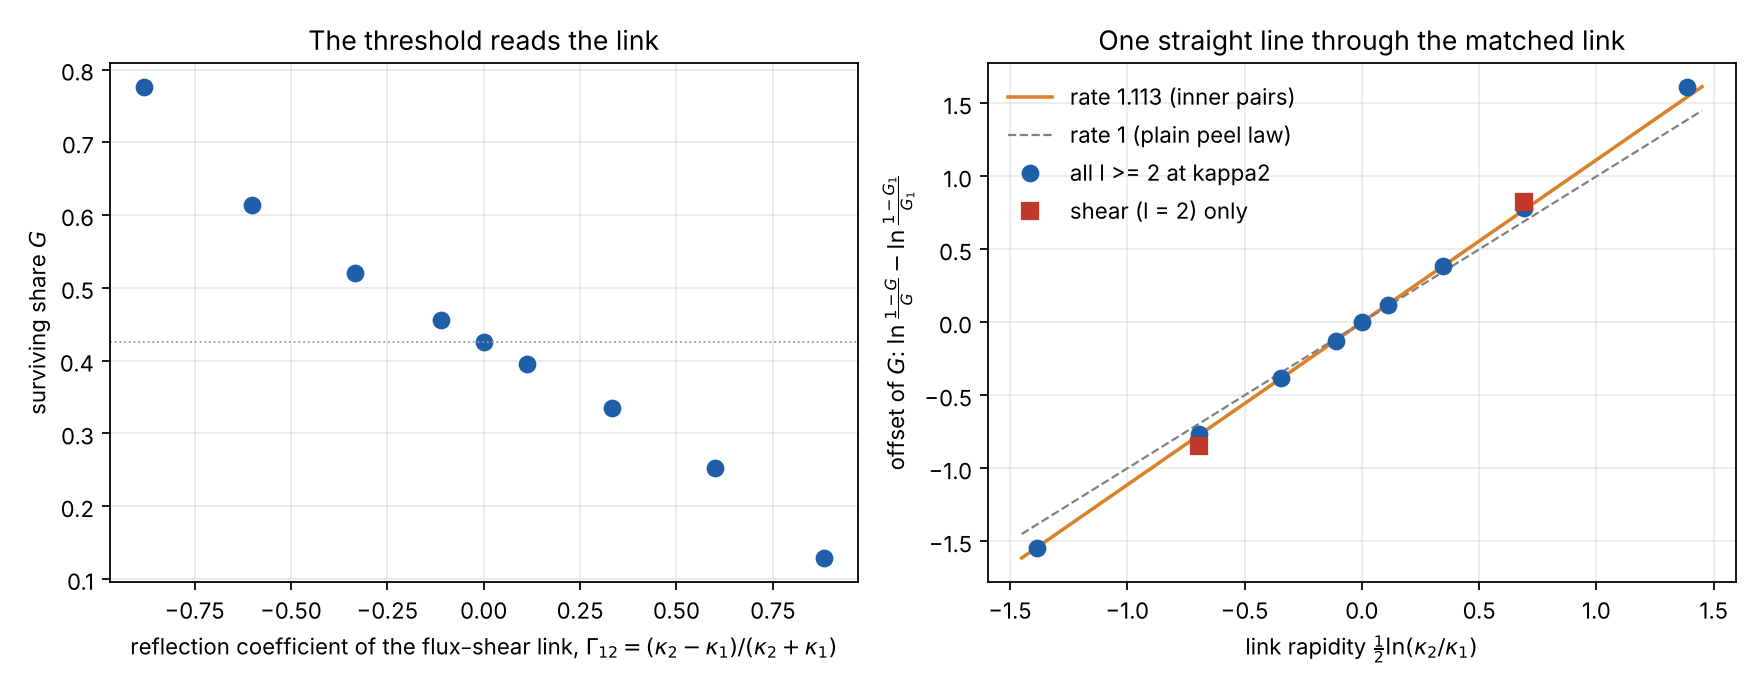
\includegraphics[width=\textwidth]{figs/fig7_link_v41.png}
\caption{The flux--shear link. Left: the surviving share $G$ against the link's reflection coefficient $\Gamma_{12}$, nine thresholds from McCormick's code with the shear and higher moments relaxing at $r$ times the flux rate. Right: the offset of $G$ against the link rapidity $\tfrac12\ln r$, with the shear-only pair (squares). Lines: rate one (dashed) and the inner-pair rate $1.113$.}\label{fig:link}\end{figure}

\paragraph{An independent check of a 3 November review.} An outside review of the companion paper reported two further thresholds on McCormick's code: a step in which collisions stop for good at $\epsilon_b=1$, at $\delta_c=0.513512$, and $n=3$, $\epsilon_{\rm dec}=1.20$, at $0.516797$. Here $0.5132$ and $0.5138$ bracket the first, and $0.5165$ and $0.5171$ the second, each dispersing below and forming a black hole above \grade{measured}.

\section{Tests for McCormick's code}

\begin{enumerate}
\item \textbf{The annihilation control.} During e$^\pm$ annihilation the plasma sound speed falls to $c_s=0.519$ at $T=0.131$\,MeV, while the neutrinos' root-mean-square speed stays $1/\sqrt3$. The contest between front and sound, $f=(1-c_s)/(1-1/\sqrt3)$, reaches $1.135$ at $1.6\times10^7\,M_\odot$ ($c_s=0.521$ there). If the softer plasma enhanced the free-streaming effect, the shift would reach $7.5\%$, outside McCormick's envelope of $5.3$--$6.2\%$, so that reading already fails. If it reduces it, the shift stays at $5.5$--$6.3\%$ \grade{computed; reading}. At $1.6\times10^7\,M_\odot$ the two readings differ from the unmodified $6.31\%$ by $+13.5\%$ and $-11.9\%$. The run McCormick lists as missing, the same transport at fixed $R_\nu$ with $p=e/3$ against the full equation of state at $3\times10^6$--$1.6\times10^7\,M_\odot$, would confirm the sign.
\item \textbf{Which mean of the rates.} McCormick calibrates his single rate to an energy-group calculation. The arithmetic mean of the group rates reproduces his calibrated decoupling temperatures: $1.62$\,MeV against $1.6$ (e$^\pm$ only), $1.02$\,MeV against $0.93$--$1.0$ (with $\nu\nu$), and a mass step of $2.53$ against $2.5$--$3$. The harmonic and geometric means fail; the mean of squares also passes, so the class of means is identified, not one mean~\cite{WB} \grade{computed; reading}.
\end{enumerate}

\section{Relation to other work}

The closest published analogue is bulk viscosity, which raises the threshold roughly in proportion to its strength in full numerical relativity~\cite{Yuwen}. Free streaming is a second dissipative channel with the same sign. Papanikolaou fixes thresholds at horizon crossing for a time-dependent equation of state, with $\delta_c$ following $c_s^2$~\cite{Pap}. Escriv\`a ties them to the initial profile and the curvature of the compaction at its peak~\cite{Esc}. Test A is consistent with both: the neutrino clock is set early.

The 2026 thermal-history mass functions through neutrino decoupling and e$^\pm$ annihilation treat neutrinos as part of the fluid~\cite{Gonin}, so the step McCormick found is absent from them. For supermassive seeds, the $\mu$-distortion bound leaves only heavy-tailed statistics~\cite{Dave}, for which McCormick finds that the raised threshold costs a factor $1.2$--$8$ in abundance in his examples~\cite{McC}.

A search of the literature to October 2026 found no other work on thresholds with free-streaming components, on gradual kinetic decoupling in numerical relativity, or on how the threshold depends on when a collision rate switches off. Tests A--D are, as far as that search shows, the first such runs.

\section{Summary}

The neutrino collision operator is a cut whose whole non-normality sits on one link, density to flux, with weight equal to the sound speed. McCormick's code, run on five cases outside his paper, shows that the collapse time alone does not set the neutrino clock, and that the decoupling history changes the threshold, not only its end point. The kept-sector memory, read mostly at the first compaction maximum and fitted once, predicted three histories it had not seen to within $0.071$, $0.014$ and $0.037$, while a history-blind rule failed. The steep-history thresholds do not move with the rate cap or the grid. The memory sits in the angular structure a fluid closure drops: set at or after decoupling, it returns into density, flux and stress; set before, it is erased. And the anisotropic stress carries the threshold: with the shear relaxing at $r$ times the flux rate, the offset of the surviving share moves close to a straight line in the link rapidity $\tfrac12\ln r$, at a rate of $1.113\pm0.007$ near the matched link, and at $1.204$ when the shear alone is damped. The direction of the flux--shear mismatch, not its connection energy, is what the collapse reads; the rate is a measured number with no closed form attached.

\begin{thebibliography}{99}
\bibitem{McC} S.~McCormick, \emph{Free-streaming neutrinos raise the threshold for primordial black hole formation}, preprint (2026). Simulation code, threshold data and scripts: Zenodo, doi:10.5281/zenodo.23808375.
\bibitem{McCcode} S.~McCormick, PBH\_neutrino\_simulation (code and threshold data), github.com/quasilocal/PBH\_neutrino\_simulation (2026); archived as doi:10.5281/zenodo.23808375.
\bibitem{CE} J.~Beasley, \emph{Non-Normality Is Connection Energy} (2026), Zenodo, doi:10.5281/zenodo.22804072.
\bibitem{WB} J.~Beasley, \emph{The Weight Between: What the present must keep, and what it costs to move it}, v1.1 (2026).
\bibitem{OSL} J.~Beasley, \emph{The Offset Speed Limit: Rate is weight}, v1.1 (2026).
\bibitem{CSL} J.~Beasley, \emph{Colour Selects the Leader}, v1.1 (2026).
\bibitem{BH} J.~Beasley, \emph{Beyond the Event Horizon: What Survives at a Rigidity Wall}, edition 10.1 (2026).
\bibitem{Rom} P.~Romatschke, \emph{Retarded correlators in kinetic theory: branch cuts, poles and hydrodynamic onset transitions}, Eur.\ Phys.\ J.\ C (2016), arXiv:1512.02641.
\bibitem{Hu} J.~Hu, \emph{Relaxation time approximation revisited and non-analytical structure in retarded correlators}, arXiv:2409.05131.
\bibitem{Yuwen} Yuwen, Joana, Wang and Cai, \emph{PBH formation with bulk viscosity}, arXiv:2606.26532 (2026).
\bibitem{Pap} T.~Papanikolaou, \emph{Toward the primordial black hole formation threshold in a time-dependent equation-of-state background}, arXiv:2205.07748.
\bibitem{Esc} A.~Escriv\`a, arXiv:2504.05814.
\bibitem{Gonin} Gonin, Froustey, Escriv\`a, Magaraggia, K\"uhnel and Hasinger, \emph{Primordial asymmetries, primordial equation of state and primordial black holes}, arXiv:2608.22240 (2026).
\bibitem{Dave} Dave, Yan, Ilyas and Cai, \emph{Evading the CMB $\mu$-distortion bound on supermassive PBH seeds with non-Gaussian tails}, arXiv:2607.03138 (2026).
\bibitem{MB} C.-P.~Ma and E.~Bertschinger, Astrophys.\ J.\ 455, 7 (1995).
\end{thebibliography}

\appendix
\section{Proofs}
\subsection*{A.1 Non-normality is connection energy, for the neutrino chain}
Let $L=A+D$ with $A^\ast=-A$ and $D^\ast=D$. Then $L^\ast=D-A$, and
\[
[L,L^\ast]=(A+D)(D-A)-(D-A)(A+D)=2(AD-DA)=2[A,D].
\]
For diagonal $D=\mathrm{diag}(D_\ell)$, $[A,D]_{ij}=A_{ij}(D_j-D_i)$. So
\[
\tfrac18\lVert[L,L^\ast]\rVert_F^2=\tfrac12\sum_{i\neq j}|A_{ij}|^2(D_i-D_j)^2 .
\]
Streaming couples only $\ell$ and $\ell\pm1$, with $|A_{\ell,\ell+1}|=kc_\ell$. Each link appears twice in the ordered sum, which gives $\sum_\ell k^2c_\ell^2(D_{\ell+1}-D_\ell)^2$. With $D=(0,-\kappa_1,-\kappa_2,-\kappa_2,\dots)$, $c_0^2=1/3$ and $c_1^2=4/15$, this is $k^2\kappa_1^2/3+\tfrac{4k^2}{15}(\kappa_2-\kappa_1)^2$. With $\kappa_1=\kappa_2=\kappa$ it is $\kappa^2k^2/3$. $\square$
\subsection*{A.2 The weight across the cut}
$PH(I-P)$ with $H=k\mu$ has the single entry $\langle0|k\mu|1\rangle=kc_0$, so $E_B=k^2/3$. The variance of $k\mu$ in the isotropic state is $k^2\langle\mu^2\rangle=k^2/3$, the same number. $\square$
\subsection*{A.3 The kept-sector propagator}
Write $u=(s-L)^{-1}|0\rangle$, so $(s+\kappa+ik\mu)u=|0\rangle+\kappa Pu$. Projecting onto $|0\rangle$ with $\langle0|(s+\kappa+ik\mu)^{-1}|0\rangle=\tfrac12\int_{-1}^{1}d\mu/(s+\kappa+ik\mu)=k^{-1}\arctan[k/(s+\kappa)]=g$ gives $u_0=g(1+\kappa u_0)$, so $u_0=g/(1-\kappa g)$. $\square$
\subsection*{A.4 The truncated exceptional point}
On $\mathrm{span}\{|0\rangle,|1\rangle\}$, $L=\begin{pmatrix}0&-ik/\sqrt3\\-ik/\sqrt3&-\kappa\end{pmatrix}$, with characteristic polynomial $\lambda^2+\kappa\lambda+k^2/3$. Its discriminant $\kappa^2-4k^2/3$ vanishes at $\kappa=2k/\sqrt3$, where the matrix is not diagonalisable. $\square$

\subsection*{A.5 Exact elimination of the hidden moments}
Write $\partial_\tau v=-(ikM+\sigma(\tau)Q)v$ with $Q=I-P$, and split $v=(a,h)$ along $P$ and $Q$. Then $\dot a=-ikc_0h_1$ and $\dot h=-(ikM_{QQ}+\sigma)h-ikc_0\,a\,e_1$. On the hidden block $\sigma(\tau)I$ commutes with $M_{QQ}$, so the generators at different times commute and the propagator is the product $U_Q(t,r)=e^{-\int_r^t\sigma}\,e^{-ik(t-r)M_{QQ}}$, with $\int_r^t\sigma=\Sigma(t)-\Sigma(r)$, $\Sigma(\tau)=-\epsilon_{\rm dec}^n/(n\tau^n)$. Variation of constants gives $h(t)=U_Q(t,s)h(s)-ikc_0\int_s^tU_Q(t,r)e_1a(r)\,dr$; substituting into $\dot a$ gives
\[
\dot a(t)=-ikc_0[U_Q(t,s)h(s)]_1-k^2c_0^2\int_s^t[U_Q(t,r)]_{11}a(r)\,dr .
\]
For two states with equal $a(s)$ the difference $\Delta a$ obeys the same equation with source $S[\Delta h(s)]$ and $\Delta a(s)=0$; if $\Delta h(s)=0$ it vanishes identically. The time-independent case $e^{t(X-\sigma I)}=e^{-\sigma t}e^{tX}$ is checked in Lean (Appendix~C). $\square$
\subsection*{A.6 The speed limit on the kept population}
With $D=-\sigma Q\le0$, $\frac{d}{d\tau}\lVert v\rVert^2=-2\sigma\lVert Qv\rVert^2\le0$, so $\lVert v\rVert\le1$ for a unit initial state. Since $\langle0|D=0$ and $\langle0|M=c_0\langle1|$, $\dot v_0=-ikc_0v_1$, and
\[
\dot A=2\,\mathrm{Re}\big(\bar v_0\,\dot v_0\big)=2\,\mathrm{Re}\big(\bar v_0(-ikc_0)v_1\big),\qquad |\dot A|\le2kc_0|v_0||v_1|.
\]
With $|v_1|^2\le\lVert v\rVert^2-|v_0|^2\le1-A$ and $k^2c_0^2=E_B$, $\dot A^2\le4E_BA(1-A)$. The core inequality $|2\,\mathrm{Re}(\bar a(-ih)b)|\le2|h||a||b|$ and the corollary under $|a|^2+|b|^2\le1$ are checked in Lean (Appendix~C). $\square$
\subsection*{A.7 Energy stationarity is not response stationarity}
Keep three moments, $\ell=0,1,2$, with streaming weights $c_0^2=1/3$, $c_1^2=4/15$ and rates $(0,\kappa_1,\kappa_2)$. The kept response $R_{00}=\langle0|(s+ikM+D)^{-1}|0\rangle$ is the continued fraction
\[
R_{00}=\cfrac{1}{s+\cfrac{k^2c_0^2}{s+\kappa_1+\cfrac{k^2c_1^2}{s+\kappa_2}}} .
\]
At $k=s=\kappa_1=1$ this is $R_{00}(\kappa_2)=\big(1+\tfrac13/(2+\tfrac{4/15}{1+\kappa_2})\big)^{-1}$, so $R_{00}(1)=32/37$ and $R_{00}'(1)=-5/1369$. The energy $E=k^2\kappa_1^2/3+\tfrac{4k^2}{15}(\kappa_2-\kappa_1)^2$ has $\partial E/\partial\kappa_2=\tfrac{8k^2}{15}(\kappa_2-\kappa_1)=0$ there. Checked by direct inversion of the $3\times3$ matrix; checked in Lean (Appendix~C). $\square$

\section{Evidence: scripts, run logs and outputs}
\subsection*{B.1 Identity checks}
\lstinputlisting{code/main/identities.py}
\lstinputlisting{code/main/identities_out.txt}
\subsection*{B.2 The one change to McCormick's code}
In a copy of \texttt{run\_nuc.py}, the collision rate line became\\
\texttt{kap = (1/(2*t))*min((eps\_dec/(2*np.sqrt(t*t0)))**nexp, kapcap)}\\
with \texttt{nexp} (default 3) and \texttt{kapcap} $=5\times10^5$ as inputs. Nothing else was changed.
\lstinputlisting{code/bisect_beyond.py}
\lstinputlisting{code/trisect_beyond.py}
\subsection*{B.3 Predictions written before the runs}
\lstinputlisting{code/PREREGISTERED.txt}
\subsection*{B.4 Run logs}
\lstinputlisting{results/log_repro.txt}
\lstinputlisting{results/log_A4.txt}
\lstinputlisting{results/log_A8.txt}
\lstinputlisting{results/log_A8b.txt}
\lstinputlisting{results/log_B2.txt}
\lstinputlisting{results/log_B3.txt}
\subsection*{B.5 Kept-sector memory curves}
\lstinputlisting{code/main/memory_curve.py}
\lstinputlisting{code/main/memory_curve_out.txt}
\subsection*{B.6 The kept-sector readings against McCormick's curve and the history prediction}
\lstinputlisting{code/wb_checks/wb_steve_03_paper_objects.py}
\lstinputlisting{code/wb_checks/wb_steve_03_out.txt}
\lstinputlisting{code/wb_checks/wb_steve_07_history.py}
\lstinputlisting{code/wb_checks/wb_steve_07_out.txt}
\lstinputlisting{results/provenance_wb07.txt}
\subsection*{B.7 Shear and flux links, and which mean of the rates}
\lstinputlisting{code/wb_checks/wb_steve_01_algebra.py}
\lstinputlisting{code/wb_checks/wb_steve_01_out.txt}
\lstinputlisting{code/wb_checks/wb_steve_04_channels.py}
\lstinputlisting{code/wb_checks/wb_steve_04_out.txt}
\subsection*{B.8 The full operator and the truncated wall}
\lstinputlisting{code/osl_checks/osl_b_ep_full_operator.py}
\lstinputlisting{code/osl_checks/osl_b_out.txt}
\subsection*{B.9 The annihilation contest}
\lstinputlisting{code/osl_checks/osl_c_speed_contest_eos.py}
\lstinputlisting{code/osl_checks/osl_c_out.txt}
\subsection*{B.10 Linear first maximum under gradual decoupling}
\lstinputlisting{code/linear_solver/lin.py}
\lstinputlisting{code/linear_solver/grad.py}
\lstinputlisting{code/linear_solver/grad.out}
\subsection*{B.11 Rate-ratio and wall readings}
\lstinputlisting{code/fixed.py}
\lstinputlisting{code/fixed_out.txt}
\lstinputlisting{code/main/lone_pass_check.py}
\lstinputlisting{code/main/lone_pass_check_out.txt}
\subsection*{B.12 Diffusive escape}
\lstinputlisting{code/csl_checks/k6_diffusion_leader.py}
\lstinputlisting{code/csl_checks/k6_diffusion_leader_out.txt}
\subsection*{B.13 Tests C and D and the controls: predictions, search script and run logs}
\lstinputlisting{code/v3_runs/PREREGISTERED_NEXT.txt}
\lstinputlisting{code/v3_runs/trisect3.py}
\lstinputlisting{results/v3/log_Bcap_part1.txt}
\lstinputlisting{results/v3/log_Bcap2.txt}
\lstinputlisting{results/v3/log_Bres.txt}
\lstinputlisting{results/v3/log_Bres2.txt}
\lstinputlisting{results/v3/log_C.txt}
\lstinputlisting{results/v3/log_D.txt}
\subsection*{B.14 The matched-pair witness}
\lstinputlisting{code/witness/PREREGISTERED_WITNESS.txt}
\lstinputlisting{code/witness/witness_run.py}
\lstinputlisting{code/witness/witness_kernel.py}
\lstinputlisting{code/witness/witness_conv.py}
\lstinputlisting{code/witness/witness_kernel.json}
\lstinputlisting{code/witness/prod.log}
\lstinputlisting{code/witness/convLM.log}
\lstinputlisting{code/witness/convTol.log}
\subsection*{B.15 The flux--shear link and the neutrino fraction: predictions, changed solver, drivers, run logs}
Every prediction and kill line of Section~\ref{sec:link} is in the file below, written before the run it judges; the results are appended under each test.
\lstinputlisting{code/v4_runs/PREREGISTERED_V4.txt}
The changed solver: McCormick's \texttt{ms\_nuc.py} (MIT licence, copyright S.~McCormick) with the collision term split (it differs from McCormick's file in its header line, the signature of \texttt{rhs}, the four lines that compute the dipole normalisation and $\kappa_2$, and the collision term), the driver that passes $r$, and the search scripts.
\lstinputlisting{code/v4_runs/ms_nuc_split.py}
\lstinputlisting{code/v4_runs/run_split.py}
\lstinputlisting{code/v4_runs/run_split_dt.py}
\lstinputlisting{code/v4_runs/trisect_fnu.py}
\lstinputlisting{code/v4_runs/trisect_split.py}
\lstinputlisting{code/v4_runs/trisect_split_dt.py}
\lstinputlisting{code/v4_runs/memory_split.py}
\lstinputlisting{code/v4_runs/memory_split_b.py}
\lstinputlisting{code/v4_runs/queue_F.sh}
\lstinputlisting{code/v4_runs/log_repro.txt}
\lstinputlisting{code/v4_runs/log_E.txt}
\lstinputlisting{code/v4_runs/log_F_regress.txt}
\lstinputlisting{code/v4_runs/log_F025.txt}
\lstinputlisting{code/v4_runs/log_F4.txt}
\lstinputlisting{code/v4_runs/log_F2a.txt}
\lstinputlisting{code/v4_runs/log_F2b.txt}
\lstinputlisting{code/v4_runs/log_H1.txt}
\lstinputlisting{code/v4_runs/log_I.txt}
\lstinputlisting{code/v4_runs/log_J2.txt}
\lstinputlisting{code/v4_runs/log_J05.txt}
\lstinputlisting{code/v4_runs/log_K125.txt}
\lstinputlisting{code/v4_runs/log_K08.txt}
The crash-safe search driver, the shear-only solver and the audit runs (Tests K repeated, L and M):
\lstinputlisting{code/v4_runs/trisect_clean.py}
\lstinputlisting{code/v4_runs/trisect_clean_res.py}
\lstinputlisting{code/v4_runs/ms_nuc_shear.py}
\lstinputlisting{code/v4_runs/run_shear.py}
\lstinputlisting{code/v4_runs/trisect_shear.py}
\lstinputlisting{code/v4_runs/queue_L.sh}
\lstinputlisting{code/v4_runs/queue_M.sh}
\lstinputlisting{code/v4_runs/log_K08_clean.txt}
\lstinputlisting{code/v4_runs/log_K125_clean.txt}
\lstinputlisting{code/v4_runs/log_L_regress.txt}
\lstinputlisting{code/v4_runs/log_L4.txt}
\lstinputlisting{code/v4_runs/log_L025.txt}
\lstinputlisting{code/v4_runs/log_M4.txt}
\lstinputlisting{code/v4_runs/log_M025.txt}
\subsection*{B.16 The check of the 3 November review}
\lstinputlisting{code/v4_runs/run_step.py}
\lstinputlisting{code/v4_runs/queue_G.sh}
\lstinputlisting{code/v4_runs/log_G.txt}
\subsection*{B.17 Figures}
\lstinputlisting{code/main/make_figures.py}
\lstinputlisting{code/main/make_figures_v3.py}
\lstinputlisting{code/main/make_fig6_door.py}
\lstinputlisting{code/v4_runs/make_fig7_link_v41.py}
\lstinputlisting{code/v4_runs/make_fig7_link_v41_out.txt}
\section{Lean statements}
\sloppy
The statements below are proved in Lean~4 with Mathlib (v4.34.1) in the repository \url{https://github.com/dicipler-pixel/neutrinos-leave-lean}. The build at commit \texttt{c372d3f} (4 November 2026) compiles every module, replays every proof in an independent kernel checker, finds that all 100 theorems of the repository use only the standard axioms (\texttt{propext}, \texttt{Quot.sound}, \texttt{Classical.choice}), and confirms that all twelve false controls are rejected. Lean checks the finite moment model and the verdict arithmetic. It does not check McCormick's code, the collapse runs, the classification of runs near threshold, the bracket edges (inputs copied from the run logs) or the numerical witness.
\begin{enumerate}
\item \texttt{crossLink}: $|2\,\mathrm{Re}(\bar a(-ih)b)|\le2|h||a||b|$; \texttt{crossLink\_sq}: with $A=|a|^2$, $|a|^2+|b|^2\le1$, the square is at most $4|h|^2A(1-A)$ (Appendix A.6).
\item \texttt{twoMomentConnectionEnergy}: $\tfrac18\lVert[L,L^\ast]\rVert_F^2=\kappa^2k^2/3$ for the two-moment $L$.
\item \texttt{splitRateEnergy}: $\tfrac18\lVert[L,L^\ast]\rVert_F^2=k^2\kappa_1^2/3+\tfrac{4k^2}{15}(\kappa_2-\kappa_1)^2$ for the three-moment $L$.
\item \texttt{shearCounterexample}: $R_{00}(1)=32/37$, $R_{00}'(1)=-5/1369$, $\partial_{\kappa_2}E=0$ at $\kappa_2=\kappa_1$; with the complex $3\times3$ resolvent entry equal to the closed form $2(15\kappa_2+17)/(35\kappa_2+39)$ for $\kappa_2>-1$ (Appendix A.7).
\item \texttt{scalarCollisionPropagator}: $e^{t(X-\sigma I)}=e^{-\sigma t}e^{tX}$, with generators $X-\sigma(t)I$ commuting pairwise (Appendix A.5).
\item \texttt{testB/C/D\_verdict}: $G_B=970/3059$, $G_C=1983/3059$, $G_D=472/3059$ against the pre-registered kill lines.
\item \texttt{gam\_inv}, \texttt{odd\_part\_free\_of\_anchor}: the link coordinate $(r-1)/(r+1)$ is odd under $r\mapsto1/r$, and the anchor cancels from the odd part (Section~\ref{sec:link}).
\item \texttt{cSq\_zero}, \texttt{cSq\_one}, \texttt{cSq\_two}, \texttt{weight\_ratio\_01}, \texttt{weight\_ratio\_12}: $c_\ell^2=(\ell+1)^2/((2\ell+1)(2\ell+3))$ gives $1/3$, $4/15$, $9/35$, and the ratios $5/4$ and $28/27$.
\item \texttt{testK\_clean\_range}, \texttt{testK\_clean\_below\_sqrt}, \texttt{testK\_clean\_above\_trend}: with the clean brackets, the innermost odd rate lies in $[1.112,1.114]$, below $1.117$ and above $1.11$; \texttt{testK\_crash\_edge\_false\_kill}: with a failed run used as a bracket edge the range would have sat wholly above $1.113$; \texttt{testK\_first\_sqrt\_window}, \texttt{testK\_first\_trend\_not\_killed}: the first clean bracket decides neither of the two readings it was set to separate.
\item \texttt{testJ\_straddles}: over its full bracket the $r=2$ odd rate straddles $1.108$ and stays at most $1.128$.
\item \texttt{testL\_rate\_ge\_six\_fifths}, \texttt{testL\_rate\_le}: the shear-only odd rate lies in $[1.2,1.21]$.
\end{enumerate}
Each verdict is a whole-number inequality: with $O(\delta)=(\delta^{\rm inst}-\delta)/(\delta-\delta^{\rm fluid})$ and $Q=O(\delta_r)/O(\delta_{1/r})$, the odd rate is at least $p/q$ exactly when $r^p\le Q^q$; $O$ decreases in $\delta$, so the two corners of the bracket pair that make $Q$ smallest and largest are the ones checked, and the kernel decides each inequality exactly.


\end{document}
